\documentclass[12pt,convert={false}]{standalone}
\usepackage[dvipsnames]{xcolor}
\usepackage{tikz}
\usetikzlibrary{shapes,arrows,positioning,calc,patterns,arrows.meta, bending, graphs, shadings,quotes,intersections}
\usetikzlibrary{external}
%\tikzexternalize[prefix=tikz/]
\usepackage{pgfplots}
\pgfplotsset{compat=1.16}
\usepgfplotslibrary{fillbetween}
\newcommand{\enf}[1]{\textcolor{RedViolet}{\textbf{#1}}} %enf sta per enfasi
\newcommand{\sott}[1]{\setulcolor{black!20!Goldenrod}\ul{#1}}
\newcommand{\prob}{\mathbb{P}}
\newcommand\independent{\protect\mathpalette{\protect\independenT}{\perp}}
\newcommand{\ev}[1]{\mathbb{E}\Bigl[{#1}\Bigr]}
\def\independenT#1#2{\mathrel{\rlap{$#1#2$}\mkern2mu{#1#2}}}
\newcommand{\Z}{\mathbb{Z}}
\newcommand{\R}{\mathbb{R}}
\newcommand{\N}{\mathbb{N}}
\newcommand{\equalexpl}[1]{%
	\underset{\substack{\uparrow\\\mathrlap{\text{\vspace{-3cm}\hspace{-1em}#1}}}}{=}}
\newcommand{\dif}{\mathop{}\!\mathrm{d}}
\begin{document}
   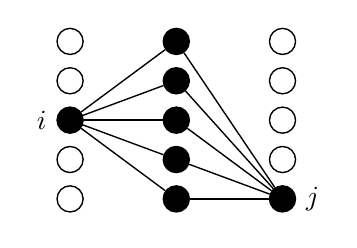
\begin{tikzpicture}[-,>=stealth', line width=0.5pt, node distance=0.5cm]
	\node [circle, draw] (zero) {};
	\node [circle, draw] (one) [below of=zero] {};
	\node [circle, draw,circle,fill=black, label=left:$i$] (two) [below of=one]{};
	\node [circle, draw] (three) [below of=two]{};
	\node [circle, draw] (four) [below of=three]{};
	
	\node [circle, draw,circle,fill=black] (a) [right=1cm of zero]{};
	\node [circle, draw,circle,fill=black] (b) [below of=a] {};
	\node [circle, draw,circle,fill=black] (c) [below of=b]{};
	\node [circle, draw,circle,fill=black] (d) [below of=c]{};
	\node [circle, draw,circle,fill=black] (e) [below of=d]{};
	
	\node [circle, draw] (f) [right=1cm of a]{};
	\node [circle, draw] (g) [below of=f] {};
	\node [circle, draw] (h) [below of=g]{};
	\node [circle, draw] (i) [below of=h]{};
	\node [circle, draw, label=right:$j$,circle,fill=black] (j) [below of=i]{};
	
	\path (two) edge node [below] {} (a);
	\path (two) edge node [below] {} (b);
	\path (two) edge node [below] {} (c);
	\path (two) edge node [below] {} (d);
	\path (two) edge node [below] {} (e);
	
	\path (a) edge node [below] {} (j);
	\path (b) edge node [below] {} (j);
	\path (c) edge node [below] {} (j);
	\path (d) edge node [below] {} (j);
	\path (e) edge node [below] {} (j);
\end{tikzpicture}
\end{document}
